\documentclass[sigconf]{acmart}

\usepackage{booktabs}
\usepackage{multirow}
\usepackage{graphicx} % Required for images
\usepackage{tikz}

\settopmatter{printacmref=true}
\renewcommand\footnotetextcopyrightpermission[1]{}
\pagestyle{plain}

\begin{document}

\title{AI for Climate Change Impact Modeling in Morocco: A Review of Applications and Opportunities}

\author{Abdelkarim Achaq}
\email{abdelkarim.achaq@usmba.ac.ma}

\author{Youness Lakhrissi}

\affiliation{%
  \institution{Faculty of Sciences and Technologies of Fez\\
  Sidi Mohamed Ben Abdellah University}
  \city{Fez}
  \country{Morocco}
}

\begin{abstract}
Morocco currently faces critical vulnerabilities driven by climate variability, manifested through intensified droughts, biodiversity loss, aquifer depletion, and coastal flooding. While Artificial Intelligence (AI) has become a global standard for climate modeling, its application within Morocco's unique Mediterranean-Saharan ecosystem requires specific contextualization. This paper presents a scoping review of 44 empirical studies (2019-2025) focusing on AI applications in three key sectors: agriculture, biodiversity, and coastal management.

Our analysis reveals that while AI models—ranging from Random Forests to Deep Learning ensembles—demonstrate high efficacy in groundwater mapping and cereal yield forecasting, significant research gaps remain. First, there is a distinct bias toward annual crops, leaving permanent crops like olive orchards under-represented despite their economic importance. Second, socio-economic dimensions remain largely unexplored, with only 9.1\% of studies incorporating human factors such as livelihoods or adaptation costs. Third, most studies rely on seasonal aggregates, missing the opportunity for real-time "early detection" of stress.

We identify a critical need for integrated AI systems that leverage cloud computing platforms (like Google Earth Engine) to bridge the gap between regional climate trends and plot-scale agricultural management. This review establishes a baseline for regionally appropriate AI climate science and highlights the urgent need for multi-disciplinary approaches in the MENA region.
\end{abstract}

\maketitle

\begin{CCSXML}
<ccs2012>
<concept>
<concept_id>10010147.10010178.10010179</concept_id>
<concept_desc>Computing methodologies~Machine learning</concept_desc>
<concept_significance>500</concept_significance>
</concept>
<concept>
<concept_id>10002951.10003317</concept_id>
<concept_desc>Information systems~Information retrieval</concept_desc>
<concept_significance>300</concept_significance>
</concept>
</ccs2012>
\end{CCSXML}

\ccsdesc[500]{Computing methodologies~Machine learning}
\ccsdesc[300]{Information systems~Information retrieval}

\keywords{Artificial Intelligence, Climate Change, Morocco, Machine Learning, Agriculture, Biodiversity, Remote Sensing}

\section{Introduction}

The Mediterranean region is warming at a rate of $0.4^{\circ}\text{C}$ per decade, surpassing global averages and intensifying the frequency of heatwaves and hydrological deficits~\cite{IPCC2021WGI}. Morocco's vulnerability is particularly acute, characterized by increasingly erratic precipitation patterns and severe water scarcity~\cite{ElKhalki2021}. The Middle East and North Africa (MENA) region as a whole is recognized as the most water-stressed globally, with Morocco's per capita water availability drastically declining from 2,560 m$^3$ per year in 1960 to approximately 620 m$^3$ in 2020, projected to fall below the absolute scarcity threshold by the end of the current decade~\cite{UNICEFWASH2023,Taheripour2020Morocco}.

\begin{figure}[t]
  \centering
  % Replace 'ghafsai_temp_trend.png' with your actual file name
  \includegraphics[width=\linewidth]{ghafsai_temp_trend.png} 
  \caption{Annual mean temperature trend (1980--2023) for the Ghafsai region derived from ERA5-Land reanalysis data. The linear regression highlights a consistent warming trajectory that directly increases evapotranspiration demands for local rainfed agriculture.}
  \label{fig:temp_trend}
\end{figure}

This warming trend is not uniform but is notably accelerated in Morocco's vulnerable agricultural zones. As shown in Figure \ref{fig:temp_trend}, the pre-Rif region (Ghafsai)—a critical area for olive production—has experienced a steady rise in mean annual temperatures over the last four decades. This historical trajectory confirms the warnings of Gumis et al.~\cite{Gumis2024} and underscores the urgent need for adaptation tools that can cope with higher evapotranspiration rates.

Globally, Machine Learning (ML) has become integral to climate adaptation strategies, offering tools to model complex non-linear environmental systems~\cite{Gumis2024,Rolnick2022TacklingCC}. A systematic analysis indicates that while classical ML remains dominant (51.4\%), deep learning approaches are rapidly gaining traction for complex tasks like weather prediction and downscaling~\cite{Ayadi2025,Alotaibi2024}.

In the Moroccan context, AI applications have expanded to include groundwater monitoring in the Saïss and Al-Haouz basins~\cite{Ragragui2024,ElMezouary2024}, crop recommendation systems~\cite{eddaoudi2023}, and coastal flood assessments~\cite{Satour2023}. However, significant gaps persist. Most research prioritizes technical metrics over socio-ecological relevance, and data scarcity in remote regions continues to hinder model transferability. This review aims to quantify these gaps and identify specific opportunities for high-impact AI interventions in the Moroccan climate context.

\section{Methodology}

We conducted a scoping review following the PRISMA-ScR guidelines to map the landscape of AI climate applications in Morocco. The process consisted of three stages:

\begin{enumerate}
    \item \textbf{Search Strategy:} We queried four primary databases (Scopus, Web of Science, ScienceDirect, and SpringerLink) covering the period from January 2019 to October 2025. The search string employed was: \texttt{("Artificial Intelligence" OR "Machine Learning" OR "Deep Learning") AND "Climate Change" AND ("Morocco" OR "North Africa")}.
    \item \textbf{Screening:} The initial search yielded 120 records. After removing duplicates (n=52) and applying inclusion criteria (empirical studies, peer-reviewed, English language), 68 records remained for abstract screening.
    \item \textbf{Selection:} Full-text analysis filtered for studies explicitly focusing on Agriculture, Biodiversity, Water Resources, or Coastal Management, resulting in a final corpus of 44 studies.
\end{enumerate}

The selection process is illustrated in Figure \ref{fig:prisma}.
\input{prisma_diagram.tex}

From each paper, we extracted data concerning the AI architectures used, data sources (satellite vs. in-situ), application sectors, and reported performance metrics.

\section{AI Techniques for Climate}

\subsection{Machine Learning Approaches}

Between 2019 and 2025, the landscape of AI-driven climate adaptation in Morocco has been dominated by Classical Machine Learning, which accounts for 51.4\% of the reviewed studies (Figure \ref{fig:ai_dist}). Among these, Random Forest (RF), Support Vector Machines (SVM), and Gradient Boosting algorithms (XGBoost, LightGBM)~\cite{Bouras2021,Ragragui2024} are preferentially selected for their robustness in handling the high-dimensional, non-linear dependencies inherent in environmental datasets. These classical methods often offer advantages in interpretability and can perform robustly even with smaller or less structured datasets, which is particularly relevant in data-scarce regions or for applications where understanding the model's decision-making process is crucial for scientific insight and trust~\cite{Jiang2024InterpretableML}.

\begin{figure}[t]
  \centering
  \includegraphics[width=\linewidth]{ai_methods_dist.png}
  \caption{Distribution of AI methodologies across the 44 reviewed studies. While classical ML (RF, SVM) remains dominant, deep learning approaches are rapidly gaining traction for complex temporal modeling.}
  \label{fig:ai_dist}
\end{figure}

Random Forest (RF) demonstrates particular efficacy in crop yield forecasting and land cover classification. Its ensemble nature mitigates overfitting—a critical advantage given the limited sample sizes often found in Moroccan agricultural studies~\cite{Bouras2021}. Prior to 2020, SVM served as the primary method for classification tasks, particularly for distinguishing vegetation types like Argan trees in the Essaouira province using multi-spectral satellite data~\cite{Rafik2023}.

More recently, Gradient Boosting algorithms have gained prominence. Bouras et al.~\cite{Bouras2021} demonstrated that XGBoost achieved superior metrics ($R^2 = 0.88$) in cereal yield forecasting compared to both RF and SVM, primarily due to its ability to model subtle residuals in complex climate-yield relationships.

\begin{table*}[!t]
\centering
\caption{Comparative Analysis of Key AI Methodologies in Moroccan Climate Applications (2019–2025)}
\label{tab:ai_methodologies}
\footnotesize
\begin{tabular}{@{}lllll@{}}
\toprule
\textbf{Algorithm} & \textbf{Category} & \textbf{Application Domain} & \textbf{Performance} & \textbf{Ref.} \\
\midrule
XGBoost & Gradient Boosting & Cereal Yield Prediction & $R^2 = 0.88$ & \cite{Bouras2021} \\
Random Forest & Ensemble & Groundwater Level (Essaouira) & NSE = 0.78 & \cite{Rafik2023} \\
Hybrid Ensemble & Stacking & Groundwater Potential (Saiss) & AUC = 86\% & \cite{Ragragui2024} \\
RF-Adaboost & Adaptive Boosting & Groundwater Potential (Tan-Tan) & AUC = 94\% & \cite{Jari2023} \\
SVM & Kernel-based & Argan Tree Classification & High Precision & El Khalki et al. \\
LightGBM & Gradient Boosting & Deforestation Monitoring & Acc = 100\% & Karmoude et al. \\
LSTM & Deep Learning & Streamflow Simulation & $R^2 = 0.84$ & \cite{AitOuchene2024} \\
MME & Neural Network & Drought Projection & Reduced Uncert. & \cite{Gumis2024} \\
\bottomrule
\end{tabular}
\end{table*}

\subsection{Deep Learning Approaches}

While classical ML remains prevalent, Deep Learning (DL) represented a paradigm shift in modeling capabilities starting around 2021~\cite{Alzubaidi2021}. The ability of Convolutional Neural Networks (CNNs) to automate feature extraction has proven invaluable for image-based tasks, such as pest detection in greenhouse crops~\cite{Esraa2025} and land cover mapping~\cite{Ragragui2024}.

For temporal data, Long Short-Term Memory (LSTM) networks have become the standard for hydrological forecasting. In the Ait Ouchene Watershed, LSTM models achieved an $R^2=0.84$ for daily streamflow simulation, effectively capturing long-term dependencies in rainfall-runoff processes~\cite{AitOuchene2024}. Furthermore, hybrid approaches like Physics-Informed Neural Networks (PINNs) are emerging. Chouaib et al.~\cite{Chouaib2025} successfully integrated physical laws into neural networks to estimate evapotranspiration (ET0) in the Tensift watershed, demonstrating that hybrid models can outperform purely data-driven approaches by respecting physical constraints.

\section{Data Sources}

\subsection{Remote Sensing and Cloud Computing}
Data scarcity remains a fundamental barrier in Morocco, a challenge echoed across many developing regions facing climate change impacts~\cite{UNICEFWASH2023}. To overcome the limitations of sparse physical monitoring networks, researchers have pivoted toward "virtual sensor networks" powered by earth observation. Studies routinely utilize Sentinel-2, MODIS, and Landsat data to derive vegetation indices (NDVI) and monitor drought stress~\cite{LePage2019}.

Crucially, the shift toward "early detection"—identifying stress before visual damage occurs—requires processing dense time-series data. Platforms like Google Earth Engine (GEE) are becoming critical in this domain. GEE allows researchers to compute high-frequency spectral indices (like NDWI or thermal anomalies) across vast temporal archives without local computational bottlenecks. This capability is essential for shifting Moroccan climate management from reactive monitoring to proactive stress mitigation~\cite{Loukili2025}.

\subsection{Ground Truth Validation}
While virtual sensors provide coverage, ground validation remains the bottleneck. High-quality labeled datasets, such as the 440 well locations used by Ragragui et al.~\cite{Ragragui2024} in the Saïss Basin, are rare, and the inherent uncertainty and logistical difficulties in acquiring precise ground truth data pose significant challenges to accurate model training and validation. Many studies are forced to rely on sparse borehole logs or limited field surveys, necessitating the use of statistical interpolation methods like Gaussian Process Regression to fill data gaps~\cite{ElMezouary2024}.

\section{Applications}

\subsection{Agriculture and Water Resources}

The agricultural sector is the focal point of AI climate research in Morocco. Applications primarily center on yield forecasting and drought monitoring. Bouras et al.~\cite{Bouras2021} developed an early warning system for cereals, achieving high predictive accuracy four months prior to harvest. Similarly, Eddaoudi et al.~\cite{eddaoudi2023} leveraged Random Forest to create accessible crop recommendation platforms.

\begin{figure*}[t] 
  \centering
  % Replace 'morocco_precip_trend.png' with your actual file name
  \includegraphics[width=\textwidth]{morocco_precip_trend.png} 
  \caption{Spatial distribution of precipitation trends (2000--2024) across Morocco based on CHIRPS satellite data. Red zones indicate a statistically significant decline in annual rainfall, confirming the widening deficit in the country's central and southern hydraulic basins.}
  \label{fig:precip_trend}
\end{figure*}

The necessity for such predictive models is driven by physical observations. Our analysis of CHIRPS satellite precipitation data (2000--2024) reveals a widespread drying trend across the Kingdom (Figure \ref{fig:precip_trend}). The severe precipitation decline in the central plains and southern basins correlates with the groundwater depletion noted by Ragragui et al.~\cite{Ragragui2024}, suggesting that future AI applications must prioritize these "red zones" where the water balance is most critical.

However, a distinct bias exists toward annual crops like cereals. Despite Morocco's status as a top global exporter of olive products, specific AI applications for permanent crops (arboriculture) remain scarce in the reviewed literature. Unlike cereals, olive orchards require year-round monitoring and specific physiological water stress indices. The lack of orchard-specific AI models represents a significant vulnerability in Morocco's adaptation strategy, particularly given the sector's reliance on increasingly scarce irrigation water.

\subsection{Biodiversity and Coastal Systems}
In biodiversity conservation, Species Distribution Models (SDMs) are identifying extinction risks. Soultan et al.~\cite{Soultan2019} projected that 17\% of endemic mammal species in the region face extinction by 2050 due to habitat shifts.
Coastal applications focus on flood resilience and marine monitoring. Satour et al.~\cite{Satour2023} utilized Self-Organizing Maps to construct a Flood Resilience Index for northern coastal regions, while other studies have deployed CNNs for jellyfish diversity monitoring in Al Hoceima Bay~\cite{Benyoub2023}.

\section{Analysis of Challenges}

\subsection{Data Scarcity and Generalizability}
Consistent with global findings~\cite{Ayadi2025}, data scarcity is the primary constraint. This is most acute in "ground-truth" availability for validation and in remote arid regions like Tan-Tan~\cite{Jari2023}. Furthermore, models trained on temperate datasets often fail to generalize to Morocco's semi-arid context, necessitating local calibration~\cite{Tramblay2013}. This contrasts with neighboring Mediterranean regions like Spain or Tunisia, where established open-data initiatives facilitate more robust model training. In Morocco, the reliance on global reanalysis products (ERA5) often introduces biases that require significant correction.

\subsection{The Granularity Gap: From Regional to Plot Scale}
While national trends are clear, a significant gap remains in detecting stress at the orchard level. Most reviewed studies operate at a coarse regional resolution. However, climate impacts are highly heterogeneous.

\begin{figure}[h]
  \centering
  % Replace 'ghafsai_stress_map.png' with your actual file name
  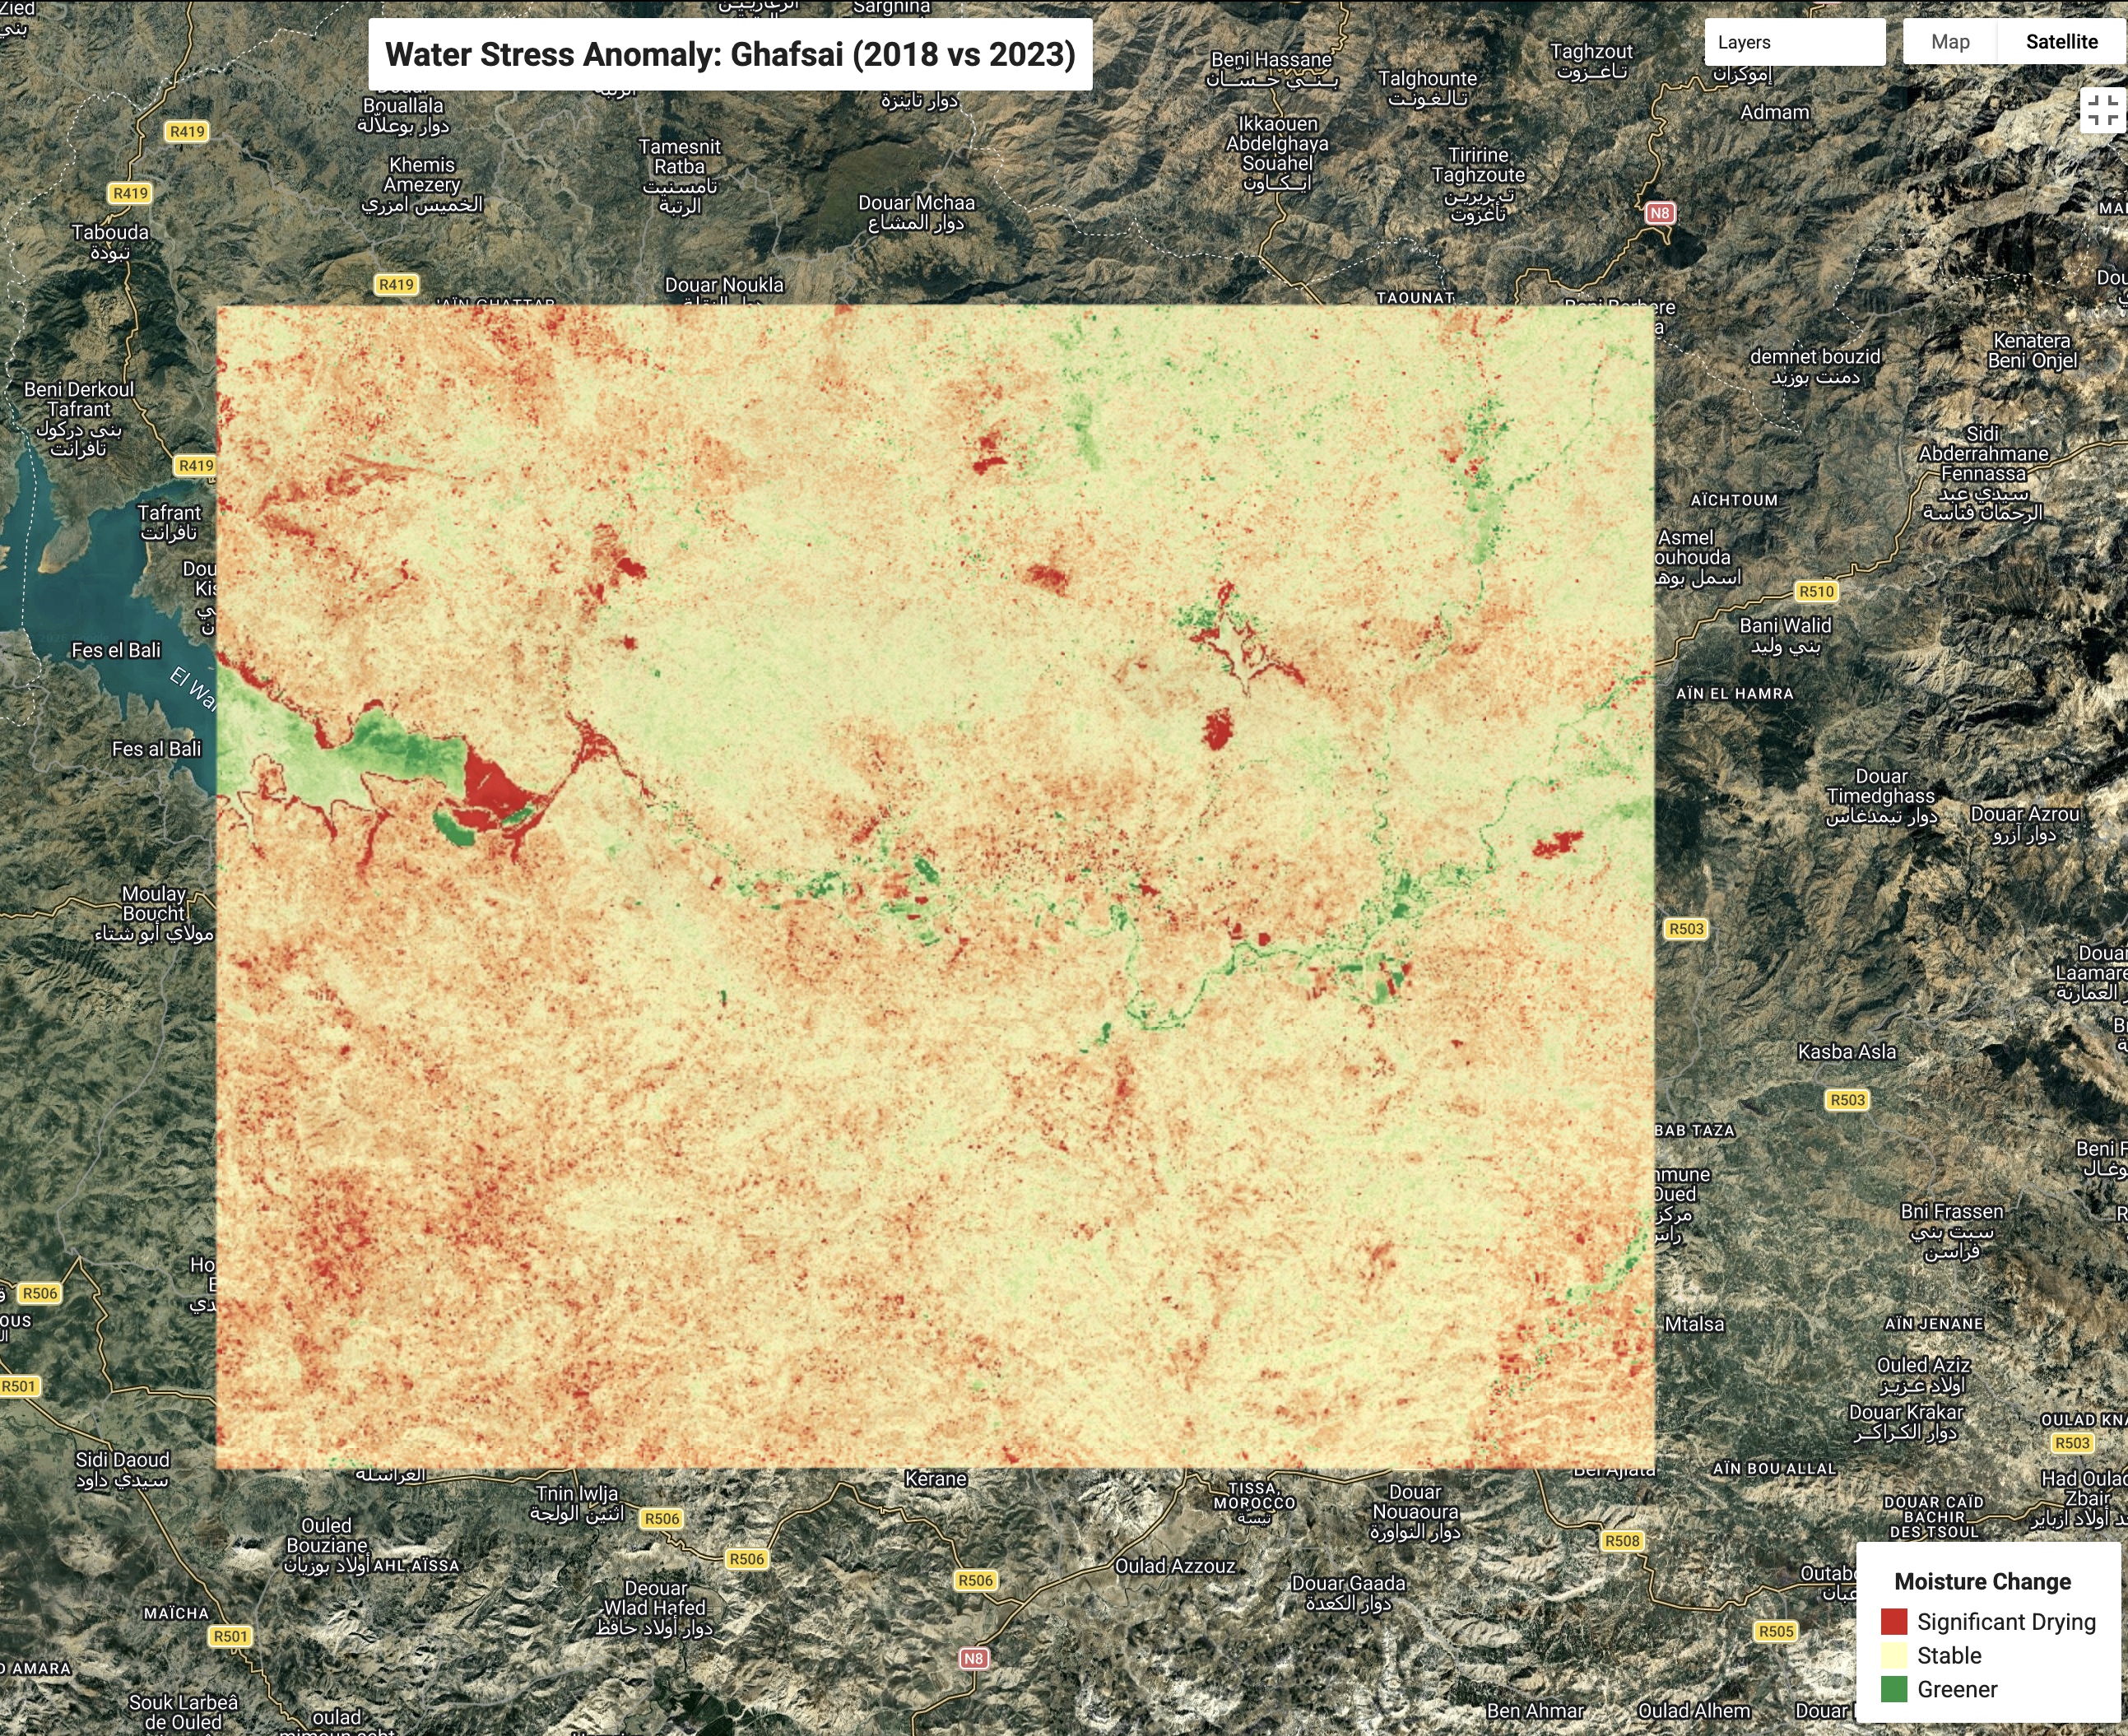
\includegraphics[width=\linewidth]{ghafsai_stress_map.png}
  \caption{Spatio-temporal analysis of moisture anomalies (NDMI) in the Taounate region (Ghafsai), comparing the 2020 baseline to the 2023 drought season. The predominance of red zones indicates widespread canopy water stress in rainfed olive orchards, illustrating the heterogeneity that current regional models often fail to capture.}
  \label{fig:olive_stress}
\end{figure}

As illustrated in Figure \ref{fig:olive_stress}, satellite analysis of the Ghafsai region reveals distinct pockets of severe water stress (NDMI anomalies) during the 2023 drought season. Current AI implementations in Morocco often lack the spatial granularity to identify these specific stress clusters in real-time, which is essential for precision irrigation in permanent crops like olive orchards.

\subsection{Lack of Socio-Economic Integration}
The most significant gap identified is the minimal integration of socio-economic factors. Only 4 out of 44 studies (9.1\%) incorporated human dimensions such as farmer livelihoods, adaptation costs, or food security. The vast majority treat climate adaptation as a purely technical engineering problem. This disconnect risks creating solutions that are technically sound but socially unimplementable, particularly for the smallholder farmers who dominate the Moroccan agricultural landscape.

\section{Recommendations}

To address the identified gaps, we propose the following strategic framework:

\begin{enumerate}
    \item \textbf{Develop National Open-Data Repositories:} Establish a centralized, open-access database for meteorological and hydrological data to reduce reliance on coarse global products.
    \item \textbf{Prioritize Permanent Crop Monitoring:} Shift research focus from annual cereals to permanent systems (olives, citrus) using high-resolution imagery (Planet, Sentinel-2) to detect orchard-level stress.
    \item \textbf{Integrate Socio-Economic Variables:} Future models must incorporate economic data (market prices, input costs) to provide actionable insights for farmers, moving beyond purely physical predictions.
\end{enumerate}

\section{Conclusion}

This scoping review analyzed the state of AI for climate impact modeling in Morocco (2019-2025). The findings highlight that while AI capabilities in groundwater mapping and cereal forecasting have matured, critical gaps impede holistic climate resilience.

We identified a "Granularity Gap," where current models fail to support permanent crop management (specifically olives) at the plot scale. Furthermore, the stark lack of socio-economic integration (9.1\% of studies) suggests that current research is disconnected from the human realities of climate adaptation.

Future research must prioritize two directions: (1) The development of GEE-based, real-time early detection systems for permanent crops that can identify stress before irreversible damage occurs, and (2) The integration of socio-economic variables into technical models to ensure that AI solutions are not just accurate, but actionable for Moroccan communities.

\bibliographystyle{ACM-Reference-Format}
\bibliography{LitReview_Conference}

\end{document}